%%%%%%%%%%%%%%%%%%%%%%% file typeinst.tex %%%%%%%%%%%%%%%%%%%%%%%%%
%
% This is the LaTeX source for the instructions to authors using
% the LaTeX document class 'llncs.cls' for contributions to
% the Lecture Notes in Computer Sciences series.
% http://www.springer.com/lncs       Springer Heidelberg 2006/05/04
%
% It may be used as a template for your own input - copy it
% to a new file with a new name and use it as the basis
% for your article.
%
% NB: the document class 'llncs' has its own and detailed documentation, see
% ftp://ftp.springer.de/data/pubftp/pub/tex/latex/llncs/latex2e/llncsdoc.pdf
%
%%%%%%%%%%%%%%%%%%%%%%%%%%%%%%%%%%%%%%%%%%%%%%%%%%%%%%%%%%%%%%%%%%%

\documentclass[runningheads,a4paper]{llncs}
\usepackage{bm}
\usepackage{amsmath}
\usepackage{amssymb}
\setcounter{tocdepth}{3}
\usepackage[pdftex]{graphicx}
\usepackage{subfigure}
\usepackage{epstopdf}
\usepackage{url}
\usepackage{hyperref}
\usepackage[boxed]{algorithm2e}
\usepackage{xcolor}

\newcommand{\di}[2]{\frac{\partial#1}{\partial#2}}
\newcommand{\trans}[1]{#1^{T}}
\newcommand{\trace}{\mathrm{tr}}
\newcommand{\diag}{\mathrm{diag}}
\newcommand{\kron}{\mathrm{kron}}

\usepackage[framemethod=TikZ]{mdframed}

\newcommand{\keywords}[1]{\par\addvspace\baselineskip
\noindent\keywordname\enspace\ignorespaces#1}
\begin{document}

%\frontmatter  % start of an individual contribution
\pagestyle{empty}
\mainmatter
% first the title is needed
\title{A Biomechanically Constrained Surface-based Registration Approach for Image-Guided Prostate Biopsy}

% a short form should be given in case it is too long for the running head
\titlerunning{A Biomechanically Constrained Surface-based Registration...}

% the name(s) of the author(s) follow(s) next
%
% NB: Chinese authors should write their first names(s) in front of
% their surnames. This ensures that the names appear correctly in
% the running heads and the author index.
%
\author{Anonymous\inst{1} \and Anonymous\inst{2} \and Anonymous\inst{3} \\ Anonymous\inst{4} \\ Anonymous\inst{5} \\ Anonymous\inst{6}}
\institute{$^1$Anonymous Institute;\\
$^2$Anonymous Institute;\\
$^3$Anonymous Institute;\\
$^4$Anonymous Institute;\\
$^5$Anonymous Institute;\\
$^6$Anonymous Institute;\\
\email{anonymous@anonymous.com}}

\newcommand{\MODIFY}[1]{\textcolor{red}{#1}}

\maketitle

\begin{abstract}
Prostate cancer (PCa) is the second most prevalent cancer in North American men. By merging information from magnetic resonance imaging (MRI) and ultrasound (US), known as MR-TRUS fusion, the cancer yield has been shown to improve for prostate biopsies. In this paper, we propose a novel surface-based registration method for MR-TRUS fusion based on Gaussian mixture models (GMM) and biomechanical regularization. Our registration framework combines the outliers/missing data rejection properties of the coherent point drift (CPD) algorithm, with a mechanically constrained internal deformation field supplied by a finite element model (FEM).  What sets our method apart from existing algorithms is a) it is very robust to noise and missing data, due to the GMM approach; and b) the FEM is included in-the-loop, which we show has a significant impact on the final deformation field.  We validate our results on data acquired from seven patients scheduled for prostatectomies. We are able to produce a mean Dice similarity coefficient of $98\%$, which is a statistically significant $8\%$ improvement compared to a typical affine registration. We also observe a mean target registration error (TRE) reduction of $0.5$~mm for targets inside the prostate. Finally, we demonstrate robustness of the method by applying it to data in which portions of the base and apex of the prostate are missing in one scan.
\end{abstract}

%%%%%%%%%%%%%%%%%%%%%%%%%%%%%%%%%
\section{Introduction}\label{sec:intro}
PCa is the second most common cancer in North American men~\cite{Cancer13a}. The definitive diagnosis of PCa relies on histology, typically from samples harvested by 2D transrectal ultrasound (TRUS)-guided core needle biopsy. It is estimated that $40\%-70\%$ of PCa tumors are isoechoic and cannot be identified using TRUS alone~\cite{Rifkin90}. Unfortunately, the current biopsy regimen is prone to false negatives, and as a result, patients with elevated prostate specific antigen levels and a negative biopsy often undergo a repeat biopsy.

Magnetic resonance imaging (MRI) has been shown to be a useful tool for PCa diagnosis~\cite{Zakian05a}. However, direct in-bore MR-guided biopsy~\cite{Xu11a} is not real-time, requires special MR-compatible equipment, and is not available in most hospitals. MR-TRUS fusion allows the information from MRI to be used to target suspicious areas invisible in US in a cost-effective manner and, as a result, to increase the cancer yield for repeat biopsy cases~\cite{Vourganti12a}.

MR-TRUS fusion is typically performed in two steps. First, just prior to the procedure, a 3D-TRUS image is generated either using a sweep across the prostate~\cite{Xu2007a} or an axial rotation of the probe around a constant pivot point~\cite{Cool11a,Sun13a}. In the second step, a pre-procedure MRI is registered to the pre-procedure 3D-TRUS~\cite{Cool11a,Sun13a,Xu2007a}. Throughout the procedure, mono-modality 2D/3D TRUS registration is used to compensate for intra-procedure motions and deformations~\cite{Silva13a}. However, the MRI is typically acquired weeks before the biopsy, in a different position (supine vs. flank), and often with an endorectal coil.  This can lead to differences in prostate shape (i.e. deformation) between MR and TRUS volumes. As a result, MR-TRUS fusion has the potential to benefit from non-rigid registration.  Furthermore, since we have the a priori knowledge that it is the same prostate in the two images, it seems reasonable to leverage this with the use of a biomechanical model.

Efficient and accurate 3D non-rigid MR-TRUS registration is inherently challenging because of the inter-modality nature of the problem and the low signal-to-noise ratio of TRUS. To the best of our knowledge, the only intensity-based approach for MR-TRUS fusion is the method by Sun~\textit{et~al.}~\cite{Sun13a}.  All other methods rely on the extraction of the TRUS surface for MR-TRUS registration~\cite{Cool11a,Hu12a,Moradi12a,Xu2007a}.  Intensity-based registration provides a direct mapping of targets inside the prostate from the MRI to the TRUS space. Although mutual information (MI) is generally used for multi-modality registrations, the differing image characteristics captured by MRI and TRUS differ to the extent where MI does not provide a good indication of image alignment. Sun~\textit{et~al.}~\cite{Sun13a} addressed this through the optimization of the modality independent neighborhood descriptor~\cite{Heinrich12a}, which is more robust to the differing intensity information provided by MRI and TRUS, but nevertheless requires some corresponding internal prostate appearance in both modalities.  This last requirement may be challenging in cases of poor clinical image quality. Since both the MR and the TRUS images are segmented during the clinical workflow to place biopsy targets within the context of the prostate boundary, we leverage this provided information as part of our method, which operates entirely independently of the interior appearance of the prostate. However, the segmentation of the boundary of the prostate apex and base can be very challenging: there is often a high variability, even among experts~\cite{Smith07a}. Therefore a method that is robust to this potential variability, or that can handle missing data in regions where the prostate boundary is not clear, would be highly valuable, as mid-gland segmentation can be done robustly and automatically.
\smallskip

\noindent\textbf{Contributions:} In this paper, we provide a novel surface-based registration method for MR-TRUS fusion based on the expectation maximization iterative closest point (EM-ICP) algorithm~\cite{Combes10a,Myronenko10a}.  It has been previously shown that these methods perform well in the presence of outliers and missing data~\cite{Myronenko10a}. Similar to~\cite{Hu12a,Moradi12a}, we constrain the registration using a FEM to regularize and limit our registration. However, our FEM is applied in-the-loop, minimizing total deformation in a continuous way throughout the iterative process.  This is in constrast to computing a deformation field in a post-processing step~\cite{Mitra12a,Moradi12a}. Moreover, our method provides a means of incorporating inhomogenous elasticity, which has been shown to improve registration further~\cite{Nir13a}. Although learning-based approaches~\cite{Hu12a} have shown promise, in this work our aim is to propose and test a method that does require a separate training phase.

%%%%%%%%%%%%%%%%%%%%%%%%%%%%%%%%%
\section{Method}
We consider the surface-based registration as a probability density estimation problem, where one surface represents the GMM centroids and the other represents observations. We use the following notations: 
\smallskip

%%%%%%%%%%%%%%%%%%%%%%%%%%%%%%%%%
\noindent\begin{tabular}{lp{0.7\textwidth}}
  \hline
  $D$ & Dimension of the point sets\\
  $X_{N\times D}$ & Observations, i.e. prostate surface points on MRI\\
  $Y_{M\times D}$ & GMM centroids, i.e. prostate surface points on US\\
  $\Phi,U$ & FEM linear interpolation matrix, nodal displacements\\
  $K$ & Stiffness matrix\\
  $P_{M\times N}$ & Posterior probabilities of GMM components\\
  $\vec{x}_{DN \times 1}$ & Rasterized representation of $X$\\
  $\diag{(\vec{v})}$ & Diagonal matrix of a vector $\vec{v}$\\
  $I$ & Identity matrix\\
  $\tilde{P} = \kron{(P,I_{D\times{D}})}$ & Kronecker tensor product of $P$ and $I_{D\times{D}}$\\
  $\vec{1}$ & Column vector of all ones\\
  \hline
\end{tabular}
%%%%%%%%%%%%%%%%%%%%%%%%%%%%%%%%%

\noindent The non-rigid registration is constrained by minimizing nodal displacements of a FEM. In place of setting boundary conditions, we drive the surface of the model using surface-to-surface forces, from model to target.  The ideal target positions are determined by a maximum a posteriori optimization problem for independent observations and can be solved by minimizing the log-likelihood function:
%%%%%%%%%%%%%%%%%%%%%%%%%%%%%%%%%
\begin{equation} \label{eq:loglike}
E(U,\sigma^2) = -\sum_{n=1}^N\log\sum_{m=1}^MP(y_m)P(x_n|y_m+\Phi_mU),
\end{equation}
%%%%%%%%%%%%%%%%%%%%%%%%%%%%%%%%%
where $\sigma^2$ is the variance of the Gaussian components.  Initially, this is set to an arbitrary large value. The objective function is optimized using an EM algorithm. In the expectation part, we compute how likely an observation corresponds to a GMM centroid by
%%%%%%%%%%%%%%%%%%%%%%%%%%%%%%%%%
\begin{equation} \label{eq:prob}
P(x_n|y_m+\phi_mU) = \frac{\exp{(-\frac{1}{2}\frac{\left\|x_n -(y_m+\Phi_mU)\right\|^2}{\sigma^2})}}{\sum_{j=1}^M\exp{(-\frac{1}{2}\frac{\left\|x_n -(y_j+\Phi_jU)\right\|^2}{\sigma^2})} + c},
\end{equation}
%%%%%%%%%%%%%%%%%%%%%%%%%%%%%%%%%
where $c=(2\pi\sigma^2)^{D/2}\frac{w}{1-w}\frac{M}{N}$ and $0{\leq}w{\leq}1$ controls the amount of outliers/missing data.
Ignoring constants independent of $U,\sigma^2$, we can rewrite the maximization step of Equation~\ref{eq:loglike} with an added FEM regularizer:
%%%%%%%%%%%%%%%%%%%%%%%%%%%%%%%%%
\begin{equation} \label{eq:obj}
Q(U,\sigma^2) = \dfrac{1}{2\sigma^2}\sum_{m,n=1}^{M,N}P(y_m|x_n)\left\|x_n- (y_m+\Phi_mU)\right\|^2 + \frac{N_PD}{2}\log(\sigma^2) +\frac{\beta}{2}\trans{\vec{u}}K\vec{u}.
\end{equation}
%%%%%%%%%%%%%%%%%%%%%%%%%%%%%%%%%
The $\beta$ parameter controls the trade-off between the tightness of the fit and regularization. Converting Equation~\eqref{eq:obj} into a rasterized form yields
%%%%%%%%%%%%%%%%%%%%%%%%%%%%%%%%%
\begin{align}\label{eq:matrixrep}
    Q(\vec{u},\sigma^2) & = \dfrac{1}{2\sigma^2}\left[ \trans{\vec{x}}\diag\left(\trans{\tilde{P}}1\right)\vec{x}+\;\trans{(\vec{y}+\tilde{\Phi}\vec{u})}\diag\left(\tilde{P}1\right)(\vec{y}+\tilde{\Phi}\vec{u})\right.\notag\\
    & \qquad\qquad \left.-2\;\trans{\vec{x}}\trans{\tilde{P}}(\vec{y}+\tilde{\Phi}\vec{u})\right] +\dfrac{N_PD}{2}\log(\sigma^2) + \dfrac{\beta}{2}\trans{\vec{u}}K\vec{u}.
\end{align}
%%%%%%%%%%%%%%%%%%%%%%%%%%%%%%%%%
This simplifies the numeric implementation. Finally, minimizing Equation~\eqref{eq:matrixrep} w.r.t $\vec{u}$ yields
%%%%%%%%%%%%%%%%%%%%%%%%%%%%%%%%%
\begin{align}\label{eq:Mstep}
        \vec{u} & = -\left[\trans{\tilde{\Phi}}\diag\left(\tilde{P}1\right)\tilde{\Phi} 
            + \beta \sigma^2K\right]^{-1}\left[\trans{\tilde{\Phi}}\diag\left(\tilde{P}1\right)\vec{y}
            -\trans{\tilde{\Phi}}\tilde{P}\vec{x}\right].
\end{align}
%%%%%%%%%%%%%%%%%%%%%%%%%%%%%%%%%
The algorithm iterates between the expectation step (updating $\sigma^2$) and maximization step (updating $\vec{u}$) until it converges to the solution. The expectation step is exactly as in Myronenko~\textit{et~al.}~\cite{Myronenko10a} and is excluded for brevity.  

Note that to form a FEM model from a surface, we often need to add interior nodes.  This can be done with most FE-meshing tools.  We create a tetrahedral mesh of the prostate, and for simplicity, we apply a homogeneous elastic material with a constant Young's modulus to all elements.  The method can be easily adapted to use non-linear, and inhomogeneous materials.

%%%%%%%%%%%%%%%%%%%%%%%%%%%%%%%%%
\begin{figure}[t]
\center
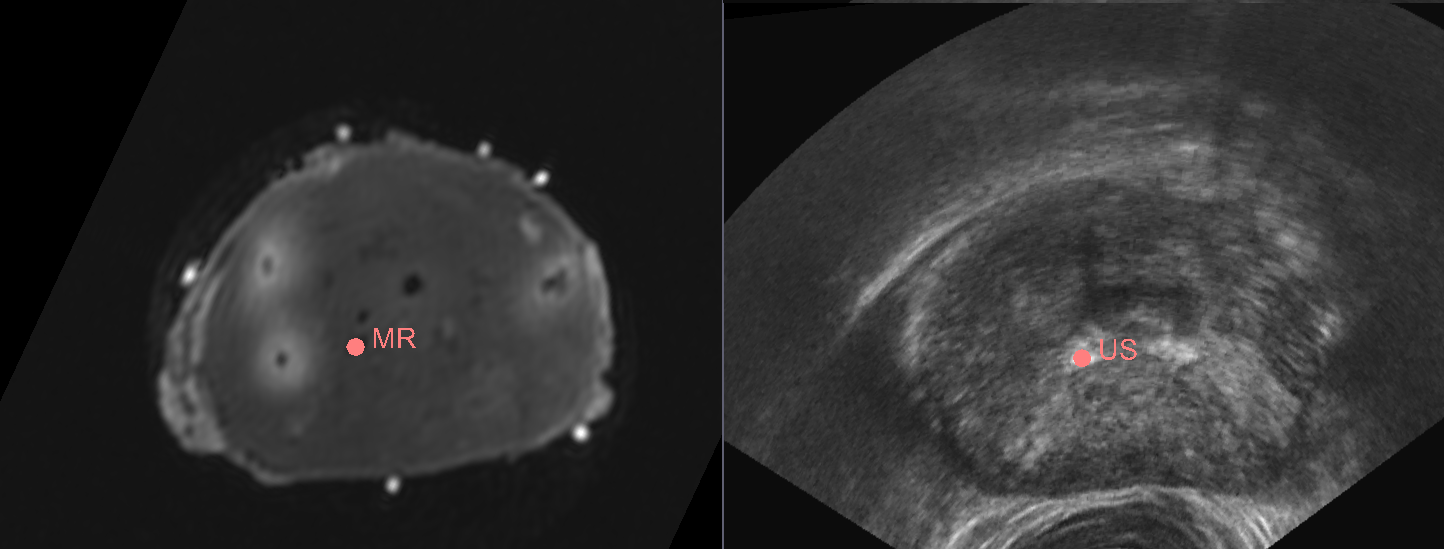
\includegraphics[width = 0.95\textwidth]{images/US_fiducial.png}
\caption{An example fiducial pair (micro-calcification) in MR (left) and US (right).}
\label{fig:fiducial}
\end{figure}
%%%%%%%%%%%%%%%%%%%%%%%%%%%%%%%%%
\section{Experiments and Results}\label{sec:exper}
This section is divided into three subsections. In Section~\ref{sec:data}, we discuss the data acquisition protocol and the registration initialization. Subsequently, we describe two sets of experiments to evaluate the performance of the proposed algorithm. In Section~\ref{sec:internal}, we investigate the internal fidelity of the deformation field using intrinsic fiducials. In Section~\ref{sec:missing}, we test robustness in the presence of missing data, which can represent uncertainty in the initial segmentation.

%%%%%%%%%%%%%%%%%%%%%%%%%%%%%%%%%
\subsection{Data}\label{sec:data}
We examine the MR and TRUS volumes from seven patients scheduled for prostatectomies. The TRUS volumes were collected with an Ultrasonix touch machine (Ultrasonix, Richmond, Canada) using a BPL-95/55 side firing transducer mounted on a motorized cradle. For this study, we opted to use the bi-planar data because probe-induced deformations are more evenly distributed. The parasagittal 2D-US images were acquired at $5^\circ$ intervals and reconstructed into a 3D-TRUS volume with an axial and lateral spacings of $0.12$~mm. Following the prostatectomy, the prostate was fixated in a $10\%$ buffered formalin solution for perservation and MR-visible strand-shaped fiducial markers were applied to the specimen using the protocol by Gibson~\textit{et~al.}~\cite{Gibson12a}. This specimen was scanned using a Discovery MR750 scanner (GE Healthcare, Waukesha, USA) at 3T using an endorectal coil (Prostate eCoil, Medrad, Warrendale, USA) to acquire T1-weighted MR images with a $0.3$~mm slice thickness. Both the MR and US volumes were manually segmented under the supervision of an expert clinican. Finally, the two segmentations were brought into an initial alignment manually, followed by an affine registration of the label maps.
%%%%%%%%%%%%%%%%%%%%%%%%%%%%%%%%%

\subsection{Internal Correctness of the Deformation Field}\label{sec:internal}
Our algorithm was implemented in Matlab (MathWorks, MA), and converges within $\approx10$~seconds on a $3.4$~GHz Intel Core i7 CPU with $8.00$~GB of RAM. In order to quantify our registration results, we used the Dice similarity coefficient to calculate the global surface-to-surface accuracy of our registration. In order to evaluate internal accuracy, we selected up to five intrinsic fiducials in the interior of the prostate per patient. Figure~\ref{fig:fiducial} shows an example of corresponding fiducial pairs (calcifications) in MR and US. The L2 norm of these fiducial pairs were used to quantify the TRE. The mean and standard deviation of the Dice coefficient, TRE, and the improvement of the TRE are shown in Table~\ref{tab:Res1}.
%%%%%%%%%%%%%%%%%%%%%%%%%%%%%%%%%
\begin{table}[tb]
\begin{center}
\caption{Mean and standard deviation of global (Dice) and local (TRE) validation metrics for the seven patients used in this study before and after FEM-based registration.}
\centering
\begin{tabular}{c| c| c| c| c| c|}
	\hline
  & \multicolumn{2}{|c|}{Dice} & \multicolumn{3}{|c|}{TRE} \\
	\cline{2-3}  \cline{4-6} 
	Metrics & Before & After & Before & After & Improvement\\
	\hline
	Values & $0.90\pm 0.02$ & $0.982 \pm 0.004$ & $3.27 \pm 1.49$ & $2.73 \pm 1.39$ & $0.54 \pm 0.32$ \\
   \hline
\end{tabular}
\label{tab:Res1}
\end{center}
\end{table}
%%%%%%%%%%%%%%%%%%%%%%%%%%%%%%%%% mean deformation 2.0
%\begin{figure}[t]
%\center
%\includegraphics[width = \textwidth]{images/TRE_diff.png}
%\caption{Histogram of improvement of the TRE for fiducial pairs following FEM-based registration.}
%\label{fig:histTRE}
%\end{figure}
%%%%%%%%%%%%%%%%%%%%%%%%%%%%%%%%%
\subsection{Effect of Missing Data}\label{sec:missing}
%%%%%%%%%%%%%%%%%%%%%%%%%%%%%%%%%
In our second study, we investigate the performance of our method when parts of the observations were missing. To this end, we removed $w$ percent of our observation points from base and apex ($w/2$ for each) and then applied our algorithm to the modified data. In order to quantify the performance in the presence of missing data, we compared the internal deformation fields with and without missing data. This is shown in Figure~\ref{fig:missingDef1}.  To highlight the significance of including the FEM-based regularization in-the-loop, we compare to another standard approach: apply a surface-to-surface registration first to estimate surface-to-surface correspondences (in our case, CPD \cite{Myronenko10a}), then use a FEM in a post-processing step to recover a volumetric deformation.  Mean differences in the resulting deformation fields are shown in Figure~\ref{fig:missingDef2}.

As shown in Figure~\ref{fig:missingDef1}, internal deformations, within one standard deviation, stay below $1.5$~mm  when $20\%$ of the data is removed. Compared to Figure~\ref{fig:missingDef2}, using surface displacements as boundary conditions for FEM-based yields larger errors when the same number of observations are removed. This suggests that continuous regularization on the internal deformation field improves the fidelity of internal mappings.

%%%%%%%%%%%%%%%%%%%%%%%%%%%%%%%%%
\begin{figure}[t]
\center
%\includegraphics[width = 0.95\textwidth]{images/combined.png}
\subfigure[]{\label{fig:missingDef1}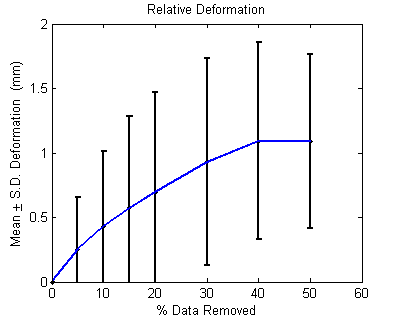
\includegraphics[width=.45\textwidth]{images/P30_ours_deformation.png}}
\subfigure[]{\label{fig:missingDef2}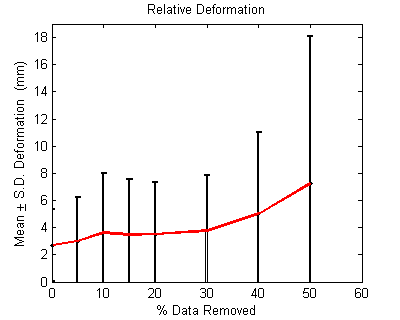
\includegraphics[width=.45\textwidth]{images/p30_CPD_deformation.png}}
\caption{Performance of FEM-based (a) and CPD (b) registration with different percentage of missing data.}
\label{fig:missingDef}
\end{figure}
%%%%%%%%%%%%%%%%%%%%%%%%%%%%%%%%%

\section{Discussion and Conclusions}

In this paper, we presented a novel surface-based registration method for MR-TRUS fusion and validated the registration result on ex~vivo MR and in~vivo US volumes acquired from seven patients. As seen in Table~\ref{tab:Res1}, following FEM-based registration, the mean Dice values improve by $8\%$. Performing a Wilcoxon rank-sum test on Dice values before and after registration shows a significant improvement ($p<10^{-4}$). This suggests that global registration evaluation metrics improve following FEM-based registration. Also, the mean TRE following FEM-based registration shows a mean improvement of $0.5$~mm. One shortcoming of our algorithm is that it requires the MR and TRUS to be segmented prior to the registration. While the MR can be segmented days ahead of time, the 3D-TRUS needs to be segmented within minutes due to clinical requirements. One possible solution is to use an existing fast segmentation method~\cite{Qiu12a}.  Of course, since the method is designed to be extremely robust to missing data, we suggest to only segment regions in which the boundary of the prostate can be clearly distinguished, such as in the mid-gland.  This can also help speed up the segmentation process.

Future work will involve registration of MR-TRUS images for patients scheduled for prostate biopsies. Since the current data was acquired using a bi-planar probe, which exerts uniform pressure throughout the prostate gland, we hope to see a larger improvement in mapping internal deformations for biopsy cases where probe pressure is variable throughout the procedure.

\bibliography{miccai.bib}
\bibliographystyle{splncs03}

\end{document}